\documentclass{homework}
\usepackage{lipsum}
\usepackage{alltt}
\usepackage{cancel}
\usepackage{amsthm}
\usepackage{cleveref}
\usepackage{upgreek}
\usepackage{mathrsfs}
\usepackage{tikz}
\usepackage{units}
\usepackage{slashbox}
\newtheorem{lemma}{Lemma}

\DeclareMathOperator{\cov}{cov}

\title{Kevin Joyce}
\course{Stat 542 - Sampling - Homework 2}
\author{Kevin Joyce}
\docdate{10 October 2014}
\begin{document} 
\newcommand{\figref}[1]{\figurename~\ref{#1}}
\renewcommand{\bar}{\overline}
\renewcommand{\hat}{\widehat}
\renewcommand{\SS}{\mathcal S}
\newcommand{\HH}{\mathscr H}
\newcommand{\mom}{\widetilde}
\newcommand{\mle}{\widehat \Uptheta}
\newcommand{\eps}{\varepsilon}
\newcommand{\todist}{\stackrel{D}\longrightarrow}
\newcommand{\toprob}{\stackrel{p}\longrightarrow} \newcommand{\TTheta}{\overline{\underline \Theta} }
\newcommand{\del}{\partial}
\newcommand{\approxsim}{\overset{\cdotp}{\underset{\cdotp}{\sim}}}
\newcommand{\RSS}{\ensuremath{\mathrm{RSS}}}
\newcommand{\MSE}{\ensuremath{\mathrm{MSE}}}
\newcommand{\SE}{\ensuremath{\mathrm{SE}}}
\newcommand{\SD}{\ensuremath{\mathrm{SD}}}
\newcommand{\TSS}{\ensuremath{\mathrm{TSS}}}
\newcommand{\Var}{\ensuremath{\mathrm{Var}}}
\newcommand{\Cov}{\ensuremath{\mathrm{Cov}}}
\newcommand{\SSReg}{\ensuremath{\mathrm{SSReg}}}
\renewcommand{\a}[1]{{\color{red} \it #1}}

\problem{ A simple random sample of 250 households was chosen from a city containing 13,828 households to estimate the proportion of households in that area who owned their home.  Of the 250 households sampled, 158 reported that they owned their home.}

\subproblem{ Estimate the population proportion of households in this city who own their home and give a \unit[99]{\%} confidence interval for this proportion. }
\begin{solution}
Let $N=13,828$, $n=250$ and $y_i = 1$ when a household from the population is owned and $0$ otherwise.  Then 
$$
  \mu = \frac 1N \sum_{i=1}^N y_i
$$
is the true population proportion we wish to estimate. Given that 158 of the households from a random sample reported ownership, we have the unbiased estimator
$$
  \bar y = \frac 1n \sum_{i=1}^n y_i = \frac {158}{250} = 0.632.
$$
One way to obtain a \unit[99]{\%} confidence interval is to invoke the Finite Population Central Limit theorem to approximate the sampling distribution of $\bar y$ with a normal distribution.  We first note that the sample variance simplifies nicely,
\begin{align*}
  s^2 = \frac{1}{n-1} \sum_{i=1}^n(y_i - \bar y)^2 = \frac 1{n-1}\left( \sum_{i=1}^n y_i^2 - n\bar y^2 \right) = \frac 1{n-1}\left( n\bar y - n\bar y^2\right) &= \frac{n}{n-1}\bar y(1-\bar y)
\end{align*}
so that we may calculate the standard error as
$$
  SE(\bar y) = \sqrt{\left(\frac{N-n}N\right) \frac{s^2}n}= \sqrt{\left(\frac{N-n}N\right)\frac{\bar y(1-\bar y)}{n-1}} \approx 0.0303.
$$
The resulting confidence interval given by $\bar y \pm t_{.995,n-1}SE(\bar y)$ is  approximately
$$
   (0.5532, 0.7108).
$$

On the other hand, we could model the exact distribution of selected owned households with a hypergeometric distribution as suggested in \emph{Thompson 5.2.}  In this case, we estimate the parameter $\tau$, the total number of owned households, where the number of owned households in an SRS follows the distribution
$$
  P(X=x|\tau) = \left.\binom \tau x \binom {N-\tau}{n-x} \middle/ \binom Nn \right..
$$
Following Thompson, for our observed $a=158$, we seek the largest $\tau_U$ such that
$$
  P(X\le a|\tau_U) > \alpha_1
$$ 
and the smallest $\tau_L$ such that
$$
  P(X\ge a|\tau_L) > \alpha_2,
$$
where $\alpha_1$ and $\alpha_2$ are such that $1-\alpha_1-\alpha_2 = .99$.  Note that the density functions for the hypergeometric for our given $N$ and $n$ are roughly symmetric for nearly all values of $\tau$, hence we choose $\alpha_1 = \alpha_2 = .005$. The resulting confidence interval is
$$
  (7609,9799)\quad\text{households}
$$
which when scaled by $\frac 1N$, gives a proportion
$$
  (0.5503,0.7086).
$$
Note that this interval generally agrees with normal approximation, but is slightly wider and centered slightly to the left of the normal one.
\end{solution}

\subproblem{ What sample size is required to estimate the proportion of people who own their own home to within 0.03 of the true proportion with \unit[99]{\%} probability.  Compute this estimate two ways: 1) using the estimate from the first sample and 2) assuming the ``worst-case.''}

\begin{solution}
  Here we assume that the sample mean \emph{is} normally distributed whose mean and variance are given exactly by our estimates $\bar y$ and $\bar y(1-\bar y)$ in part (a).  Under this assumption, setting the theoretical margin of error
  $$
    z\sqrt{\left(\frac{N-n}{N}\right) \frac{\bar y(1-\bar y)}{n}} = d = 0.03
  $$
  implies 
  $$
    n = \left( \frac 1{n_0} + \frac 1N \right)^{-1}
  $$
  where $z$ is the $.995$ quantile of the standard normal distribution and
  $$
    n_0 = \frac{z^2 \bar y(1-\bar y)}{d^2} \approx  1714.575
  $$
  So $n$ is at least 
  $$
    \left( \frac 1{n_0} + \frac 1N \right)^{-1} \approx 1525.432 \implies n\ge 1526.  
  $$  
  If we do not take into account the previous study, but make the same distributional assumptions, then the necessary $n$ is maximized when $n_0 \propto \bar y(1-\bar y)$ is maximized which occurs when $\bar y = \frac 12$, so $\sigma_{max}^2 = \frac 14$.  This results in 
  $$
    \left( \frac{4 d^2}{z^2} + \frac 1N \right)^{-1} \approx 1626.27 \implies n_{max}\ge 1627.
  $$
\end{solution}
\newpage
\problem{ \emph{Thompson 6.3.}  In a water pollution study, a sample of lakes is selected from the 320 lakes in a study region by the following procedure.  A rectangle of length $l$ and width $w$ was drawn around the study region on a map.  Pairs of random numbers between $0$ and 1 were generated from the uniform distribution using a random number generator on a computer.  The first random number of a pair was multiplied by $l$ and the second by $w$ to give location coordinates within the study region.  If the location was in a lake, that lake was selected.  This process was continued until four of the points had fallen on lakes.  The first lake in the sample was selected twice by this process, while each of the other two were selected just once.  The pollutant concentrations (in parts per million) for the three lakes in the sample were 2, 5, and 10.  The respective sizes of the three lakes (in \unit{km\textsuperscript2}) were 1.2,0.2, and 0.4. In all, \unit[80]{km\textsuperscript2} of the study region was covered by lakes. }

\subproblem{ Describe concisely the type of design used.  }
\begin{solution}
  In this study the population is each lake enclosed in the rectangle on the
  map where a lake is a sampling unit.  The response unit, $y_i$, is
  pollutant concentraion. The sampling units have \emph{unequal} probability of
  selection.  Assuming the points follow a bivariate uniform distribution, the
  probability of selection of a given lake is its area on the map divided by
  $w\times l$.  The sampling is done \emph{with} replacement.  Concicely, this is PPS with replacement.
\end{solution}

\subproblem{ Give an unbiased estimate of the mean pollution concentration per lake in the population. Show how to get the answers selected in the back of the book. }
\begin{solution}
  The back of the book uses the Hansen-Hurwitz estimator for the mean.  This is computed as follows:
  $$
    \hat\mu_p = \frac 1N \hat \tau_p = \frac 1{N} \frac 1n \sum_{i=1}^n \frac {y_i}{p_i} = \frac 1{320}\frac14 \left( \frac{2}{1.2/80} +\frac{2}{1.2/80} +\frac{5}{0.2/80} + \frac{10}{0.4/80} \right) \approx  3.02\text{ parts per million }
  $$
\end{solution}

\subproblem{ Estimate the variance of the estimator above. }
\begin{solution}
  The variance estimator for Hansen-Hurwitz is given by
  \begin{align*}
    \frac 1{N^2} \hat{\Var}(\hat\tau_p) 
    &= \frac 1{N^2n(n-1)} \sum_{i=1}^4 \left(\frac{y_i}{p_i} - N\hat\mu_p\right)^2\\
    &= \frac 1{320^2\cdot 4 \cdot 3} \left\{\left(\frac{2}{1.2/8} - N\hat\mu_p\right)^2+\left(\frac{2}{1.2/8} - N\hat\mu_p\right)^2 \right.\\
    &\quad...\left.+\left(\frac{5}{0.2/8} - N\hat\mu_p\right)^2+\left(\frac{10}{0.4/8} - N\hat\mu_p\right)^2\right\}\\
    &\approx 2.33\text{ (part per million)}^2.
  \end{align*}
\end{solution}

\problem{ \emph{Thompson 6.3.Modified.} Suppose you don't know the total number of lakes in the study region nor the total area covered by the lakes.  Estimate the mean pollution concentration per lake and the mean size of the lakes in the region.  Compute standard errors and confidence intervals for both estimates by two methods: linearization and bootstrapping (note: the sample size here may be too small for either of these methods to work well). }
\begin{solution}
If we take $x_i$ to be the area of the lake sampled in \unit{km} as an auxiliary variable and $y_i$ to be the pollution concentration in parts per million as before, then a biased estimator for $\mu_y$ is given by estimating the total pollution in each lake and dividing by an estimate for the total number of lakes; i.e.
$$
  \hat \mu_y = \frac{\hat \tau_y}{\hat N} = \frac{\ds{\sum_{i=1}^4\frac{y_i}{x_i}}}{\ds{\sum_{i=1}^4\frac{1}{x_i}}} = \frac{\ds{\frac{2}{1.2} +\frac{2}{1.2} +\frac{5}{0.2} + \frac{10}{0.4}}}{\ds{\frac{1}{1.2} +\frac{1}{1.2} +\frac{1}{0.2} + \frac{1}{0.4}}}\approx  5.577\text{ ppm per lake}
$$ 
where we cancel $\tau_x$ and $\frac 1n$ from the numerator and denominator. Let $t_i = y_i/x_i$ and $v_i = 1/x_i$, then $\hat \mu_y$ is a ratio estimator and an estimate of its variance is given by (ignoring the finite population correction)
$$
  \hat{\Var}(\hat \mu_y) = \frac{1}{\bar v^2} \frac{s_r^2}{n}\text{ where }s_r^2 = \frac{1}{n-1}\sum_{i=1}^n(t_i - \hat \mu_y v_i)^2
$$
whose square root gives
$$
  \SE(\hat \mu_y) \approx 1.361\text{ ppm per lake. }
$$
A \unit[95]{\%} confidence interval is given by
$$
  \hat\mu_y \pm t_{.975,3} SE(\hat \mu_y)\quad\text{approximately} \quad (\,1.246\,,\, 9.908\,)\text{ ppm per lake.}
$$
\begin{minipage}{.5\textwidth}
If, on the other hand, we bootstrap the sample with $N=10^5$ resamples, we obtain the output
{\footnotesize
\begin{verbatim}
Bootstrap Statistics :
    original      bias    std. error
t1* 5.576923 -0.05955984    1.504699
\end{verbatim}
}
and proportional and BCa confidence intervals
{\footnotesize
\begin{verbatim}
Level     Percentile            BCa          
95%   ( 2.000,  9.024 )   ( 2.000,  9.024 )  
\end{verbatim}
}
Note the relatively sparse histogram due to the low sample size.
\end{minipage}
\begin{minipage}{.48\textwidth}
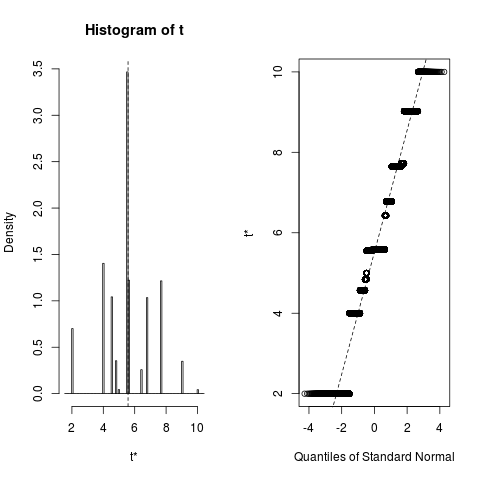
\includegraphics[width=\textwidth]{pollution_bootstraps.png}
\end{minipage}

Thinking of the response as $y'_i = 1$ for each lake, then the Hansen-Hurwitz estimator $\sum_{i=1}^n\frac{y'_i}{p_i}$ is an ubiased estimator for $\tau_{y'_i} = N$. Denote that estimator as $\hat N$, then we can also estimate the average lake size since
$$
  \hat\mu_x = \frac{\tau_x}{\hat N} = \frac{\cancel\tau_x}{\ds{\frac 1n\sum_{i=1}^n\frac{1}{x_i/\cancel{\tau_x}}}} = \frac{1}{\ds{\frac 1n\sum_{i=1}^n\frac{1}{x_i}}} \approx \unit[0.462]{\mathrm{km}^2}
$$
and by linearizing $\frac 1{\bar v}$ where $v_i = \frac 1{x_i}$, we can estimate the linearized variance
$$
  \Var(\hat\mu_x) \approx \left(\frac{1}{\bar v^4}\right) \frac{\sigma^2_v}{n}
$$ with (again ignoring the finite population correction factor)
$$
  \hat{\Var}(\hat\mu_x) = \left(\frac{1}{\bar v^4}\right) \frac{s^2_v}{n}
$$
which gives
$$
  \SE(\bar\mu_x) \approx \unit[0.210]{\mathrm{km}^2}.
$$
A \unit[95]{\%} confidence interval is given by
$$
  \hat\mu_y \pm t_{.975,3} \SE(\hat \mu_y)\quad\text{approximately} \quad ( \,-0.205\,,  1.128\,)\,\mathrm{km}^2.
$$

Note that $\hat\mu_x$ is likely not a great estimator since our estimate of $\SE(\hat\mu_x)$ is quite large and the interval contains negative values which makes no physical sense.

\begin{minipage}{.5\textwidth}
When we bootstrap the sample with $N=10^5$ resamples, we obtain the output
{\footnotesize
\begin{verbatim}
Bootstrap Statistics :
     original     bias    std. error
t1* 0.4615385 0.08908693   0.2517804
\end{verbatim}
}
and proportional and BCa confidence intervals
{\footnotesize
\begin{verbatim}
Level     Percentile            BCa          
95%   ( 0.2526,  1.2000 )   ( 0.2000,  0.8889 )  
\end{verbatim}
}
Note the non-symmetry in the histogram. Also, both the bias corrected and the resampling percentile intervals do not contain negative values like the linearized interval.  Here is a situation where bootstrapping seems to be a better choice than linearization.

\end{minipage}
\begin{minipage}{.48\textwidth}
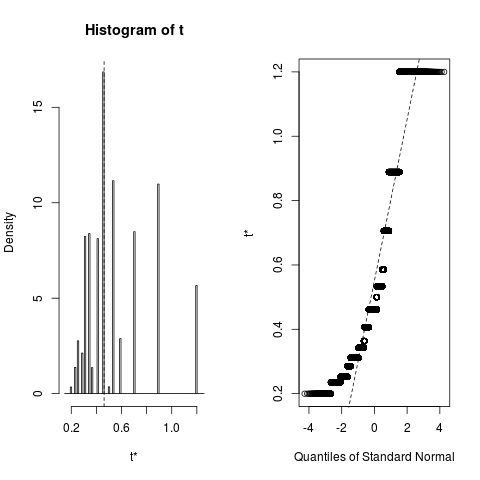
\includegraphics[width=\textwidth]{mean_lake_bootstraps.png}
\end{minipage}

\end{solution}
\newpage 

\problem{ \emph{Thompson 7.5.} Determine the first- and second-order terms of a Taylor series expansion of the ratio estimator.  Use the approximation to obtain an approximate expression for the bias of the ratio estimator under simple random sampling. }
\begin{solution}
  The ratio estimator as a function of the sample means is
  $$
    f(\bar x, \bar y) = \frac{\bar y}{\bar x},
  $$
  whose second-order Taylor series expansion about $(\mu_x,\mu_y)$ is
  \begin{align*}
    f(\bar x, \bar y) 
    &= f(\mu_x,\mu_y) + f_{\bar x}(\mu_x,\mu_y) (\bar x-\mu_x) + f_{\bar y}(\mu_x,\mu_y)(\bar y - \mu_y) \dots\\
    &\dots + \frac 12\left( f_{\bar x \bar x}(\mu_x,\mu_y) (\bar x - \mu_x)^2 +  f_{\bar y \bar y}(\mu_x,\mu_y) (\bar y - \mu_y)^2  + 2f_{\bar x\bar y}(\mu_x,\mu_y)(\bar x-\mu_x)(\bar y-\mu_y)\right) + R_{\mu_x,\mu_y}\\
    &= \frac{\mu_y}{\mu_x} - \frac{\mu_y}{\mu_x^2}(\bar x-\mu_x) + \frac{1}{\mu_x}(\bar y - \mu_y) \\
    &\dots + \frac 12\left( \frac{2 \mu_y}{\mu_x^3}(\bar x - \mu_x)^2 +  \cancel{0 (\bar y - \mu_y)^2}  - 2\frac{1}{\mu_x^2}(\bar x-\mu_x)(\bar y-\mu_y)\right) + R_{\mu_x,\mu_y}.
  \intertext{ Taking the expected value of both sides, and dropping $E \Big[R_{\mu_x,\mu_y}(\bar x, \bar y)\Big]$, we obtain }
    E \frac{\bar y}{\bar x} 
    &\approx \frac{\mu_y}{\mu_x} - 0 + 0 + \frac{\mu_y}{\mu_x^3} E(\bar x - \mu_x)^2 - \frac{1}{\mu_x^2} E\Big[(\bar x - \mu_x)(\bar y -\mu_y)\Big].
  \end{align*}
  So an approximation of the bias of the ratio estimator $r=\frac{\bar y}{\bar x}$ is
  $$
    E\frac{\bar y}{\bar x} - \frac{\mu_y}{\mu_x} \approx \frac{\mu_y}{\mu_x^3} \Var(\bar x)- \frac{1}{\mu_x^2} \Cov(\bar x, \bar y).
  $$
\end{solution}

\problem{ Omitted }

\problem{ The file \texttt{census.csv} has data on a number of variables for all 3143 countries in the U.S.~from the 2010 U.S.~Census.  You can read it into \texttt R using the \texttt{read.csv} command.  This will create a data frame in \texttt R. For this exercise, we are only interested in two variables: \texttt{TotalPop}, the total number of persons counted in the country, and \texttt{HousingUnits}, the total number of housing units (both owned and rented) in the country.  Suppose we are interested in seeing if we can accurately estimate the total number of people in the U.S.~by counting the number of housing units in every county, which we think will be much easier than trying to count every person (including the homeless).  Our plan is then to take a sample of counties where we will do a careful count of all the people living there and then extrapolate to the U.S.~using ratio or regression estimation.  Note that we have the entire population so we can see well these methods work for possible use in the next decennial Census in 2020. }  

\subproblem{ Examine the relationship between number of housing units and total population for all counties in the U.S.~with a scatterplot.  Does it appear that using number of housing units as an auxiliary variable through ratio or regression estimator might be helpful in estimating the total population of the U.S.?}
\newpage
\begin{solution}
  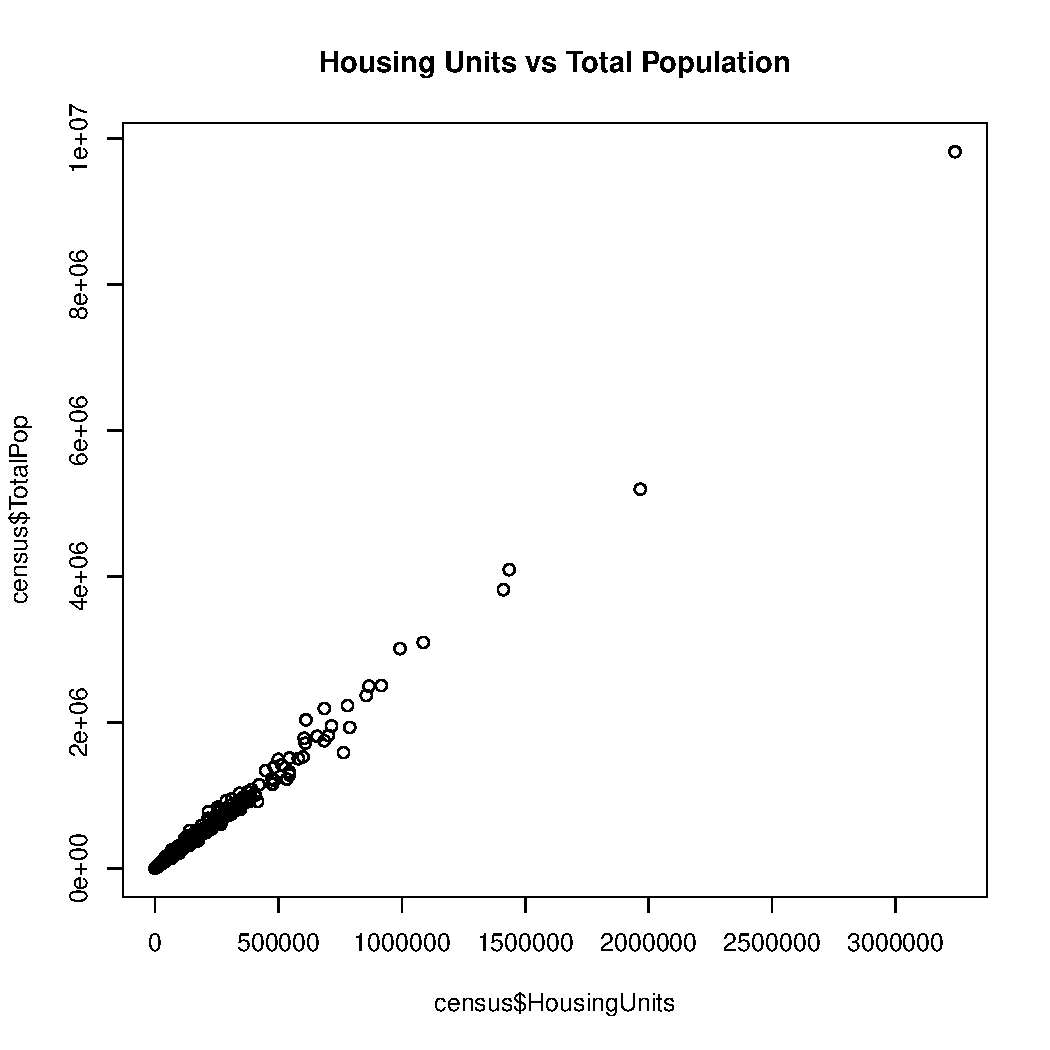
\includegraphics[width=.45\textwidth]{house_pop_compare.pdf}
  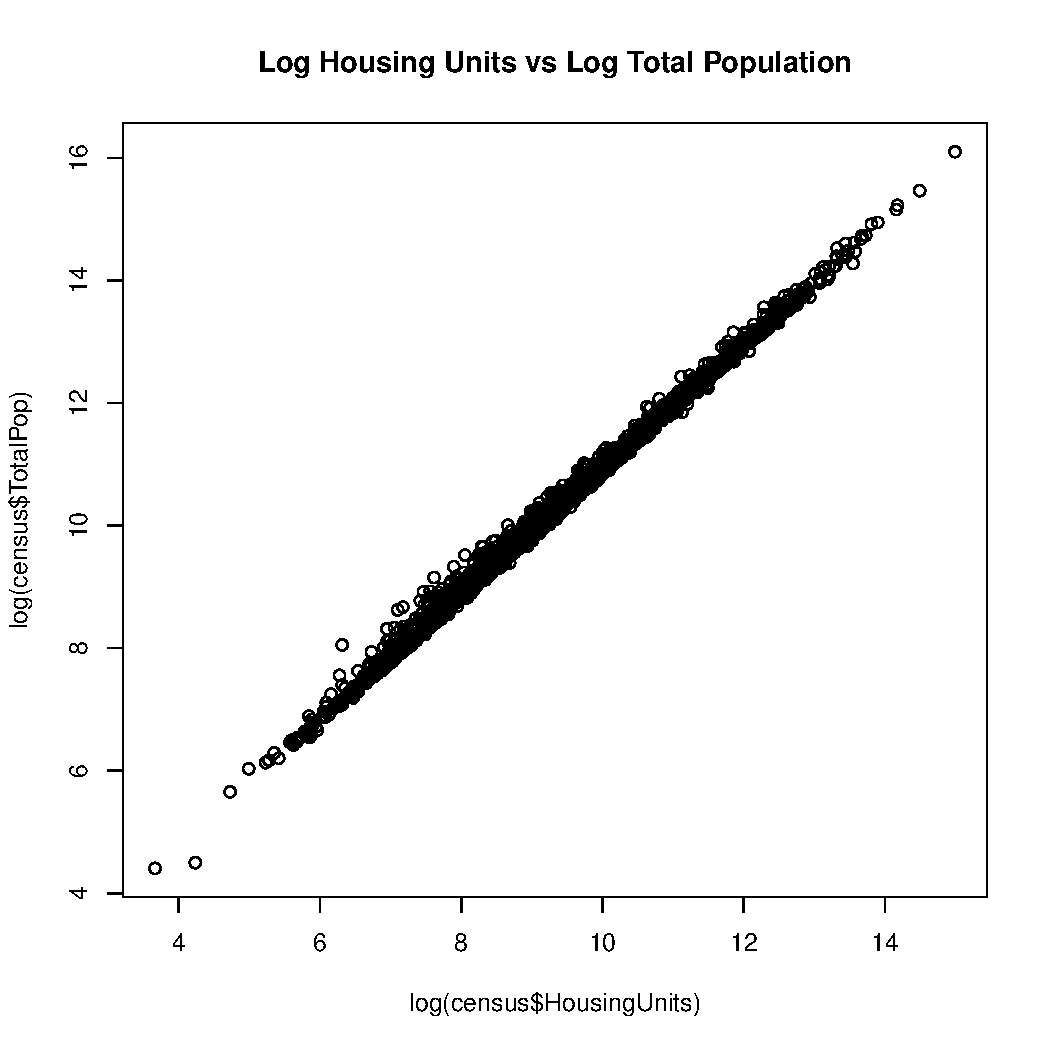
\includegraphics[width=.45\textwidth]{log_compare.pdf}

The plot on the left plots the total population of each county versus the
housing units in each county.  The plot on the right plots these variables both
on a log scale, which makes the linear relationship for smaller counties easier to see (the slope is close to \emph{one}).
These suggest that either ratio or regression estimation is appropriate.
\end{solution}

\subproblem{ Set up a script in \texttt{R} to draw an SRS of 100 counties and
compute three estimates of the total population of the U.S.: the simple SRS
estimate without using an auxiliary variable, and the ratio and regression
estimates by using the total number of housing units in the country as an
auxiliary variable. Draw a few different samples and see how the estimates
compare to the true value (which you can calculate from the data frame using
the \texttt{sum} command.)  Which appears to be doing best?  You do not need to
report numerical results for this part; just report what you observe. }

\begin{solution} 
  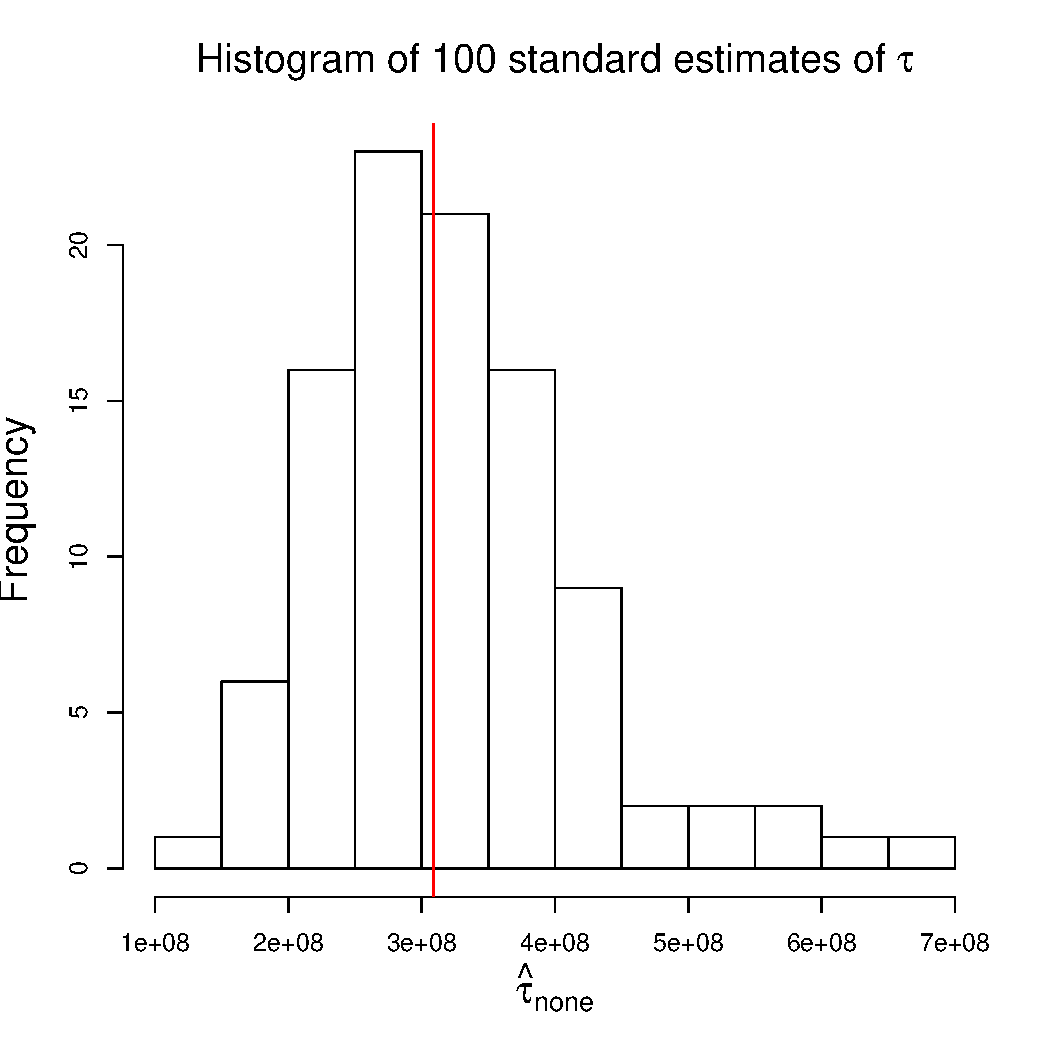
\includegraphics[width=.3\textwidth]{none_hist.pdf}
  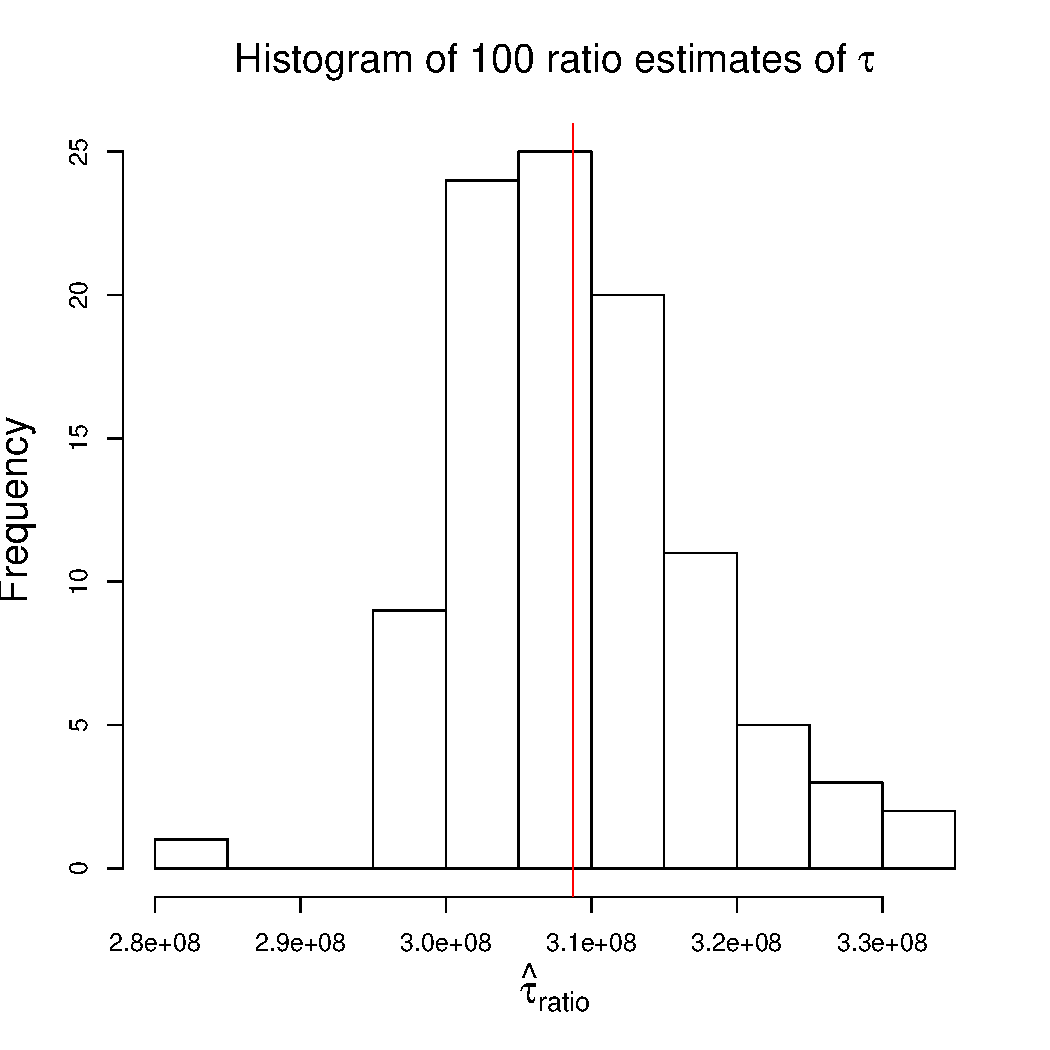
\includegraphics[width=.3\textwidth]{ratio_hist.pdf}
  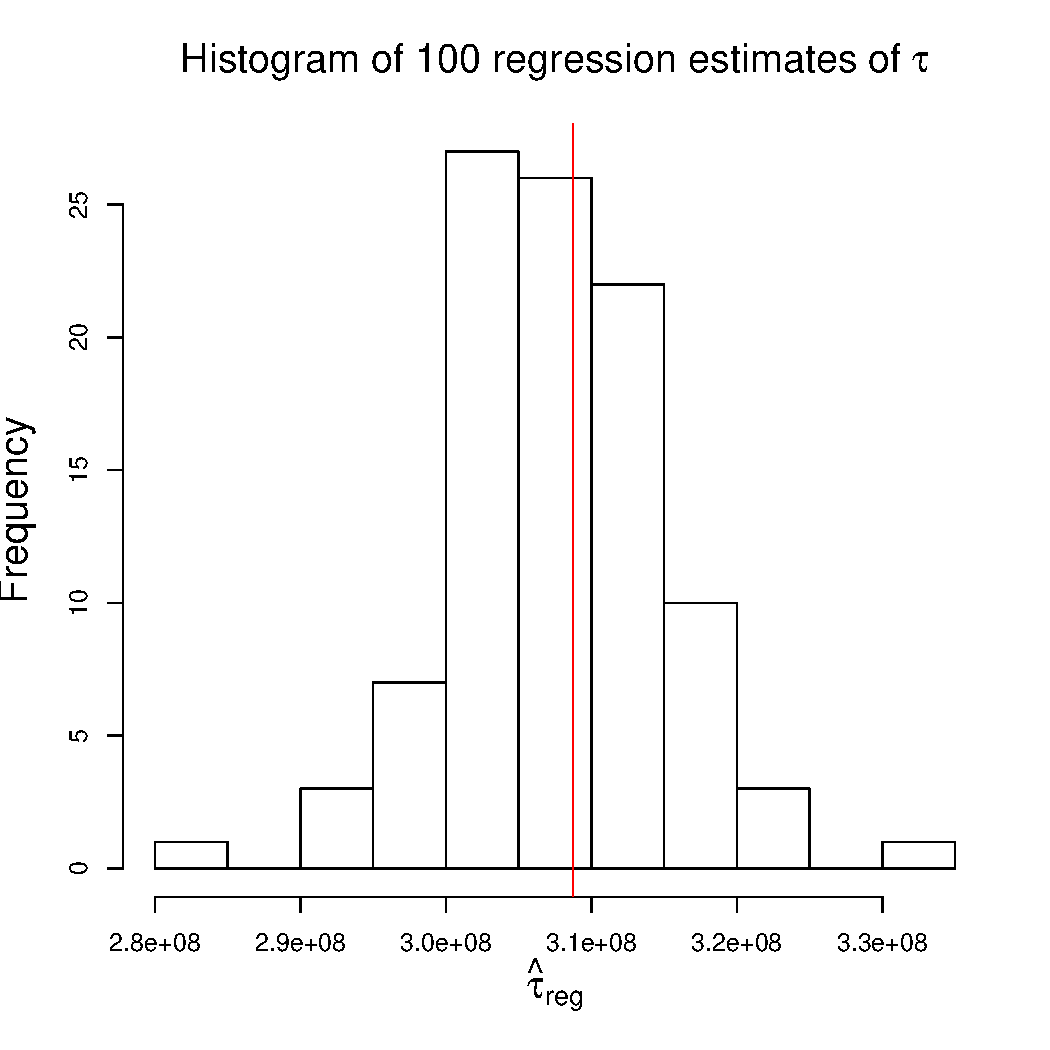
\includegraphics[width=.3\textwidth]{regression_hist.pdf}
\end{solution}

The above histograms summarize each of the three estimates on 100 random
samples.  The true total population is indicated by a red line in each plot.
Both the ratio and regression estimators seem to perform better in terms of
precision (they are spread out less).  Compared to each other, they are mostly
indistinguishable from these plots.

\subproblem{ To mimic what would happen in practice, take an SRS of size $n=100$ and compute the three estimators and their standard errors (using the finite population correction).  Before you select your sample, use the \texttt R command \texttt{set.seed()} where you put any integer inside the parenthesis to set the random number generator so I can reproduce your sample and check your calculations (e.g., \texttt{set.seed(45519)}).}
\begin{solution}

A summary of the calculations is given for the given seed below.  Note that these results reflect the samples done in part (b) -- that is the standard error without the auxilary information is much higher. 
%Using the formulae
%$$
%  \hat{\Var}(\hat\tau_{none}) = \left(1-\frac nN\right) \frac {s^2}{n}
%  \quad
%  \hat{\Var}(\hat\tau_{ratio}) = \left(1-\frac nN\right) \frac{s^2_r{n}
%  \quad
%  \hat{\Var}{\hat\tau_{regression}} = 
%$$
\begin{center}
\renewcommand{\arraystretch}{1.3}
\begin{tabular}{c| r r r}
		      &      none  &     ratio &  regression\\ \hline
$\hat{\tau}$          &  276911626 & 303769175 &   304761946\\
$\hat{\SE}(\hat\tau)$ &   54664378 &   6261614 &     5984781\\
\end{tabular}
\end{center}

\end{solution}

\subproblem{ Since we have the entire population, we can calculate the theoretical standard deviation of the sample mean and the approximate theoretical standard deviations of the ratio estimator and regression estimators.  Go ahead and do so. }
\begin{solution}

(Thanks to Grant Swicegood for troubleshooting this with me.) In the following table we summarize the calculations of the true (approximate when relevant) sample standard errors.  We also compare these with the sample estimates by dividing our estimates for $\hat{\SE}(\hat\tau)$ by $N$.  Note that each estimate drastically underestimates the true value.
\begin{center}
\renewcommand{\arraystretch}{1.3}
\begin{tabular}{c| r r r}
		      &      none &    ratio & regression\\\hline
$\SE(\hat\mu)$       &  30788.32 & 3181.354 &   2797.085\\
$\hat{\SE}(\hat\mu)$ &  17392.42 & 1992.241 &   1904.162\\\hline
$\SE(\hat\tau)$       & 96767696 & 9998995 &    8791238\\
$\hat{\SE}(\hat\tau)$ & 54664378 & 6261614 &    5984781\\
\end{tabular}
\end{center}

If we simulate more samples and observe the histogram of these estimates,
similar to part (b), we obtain: 

  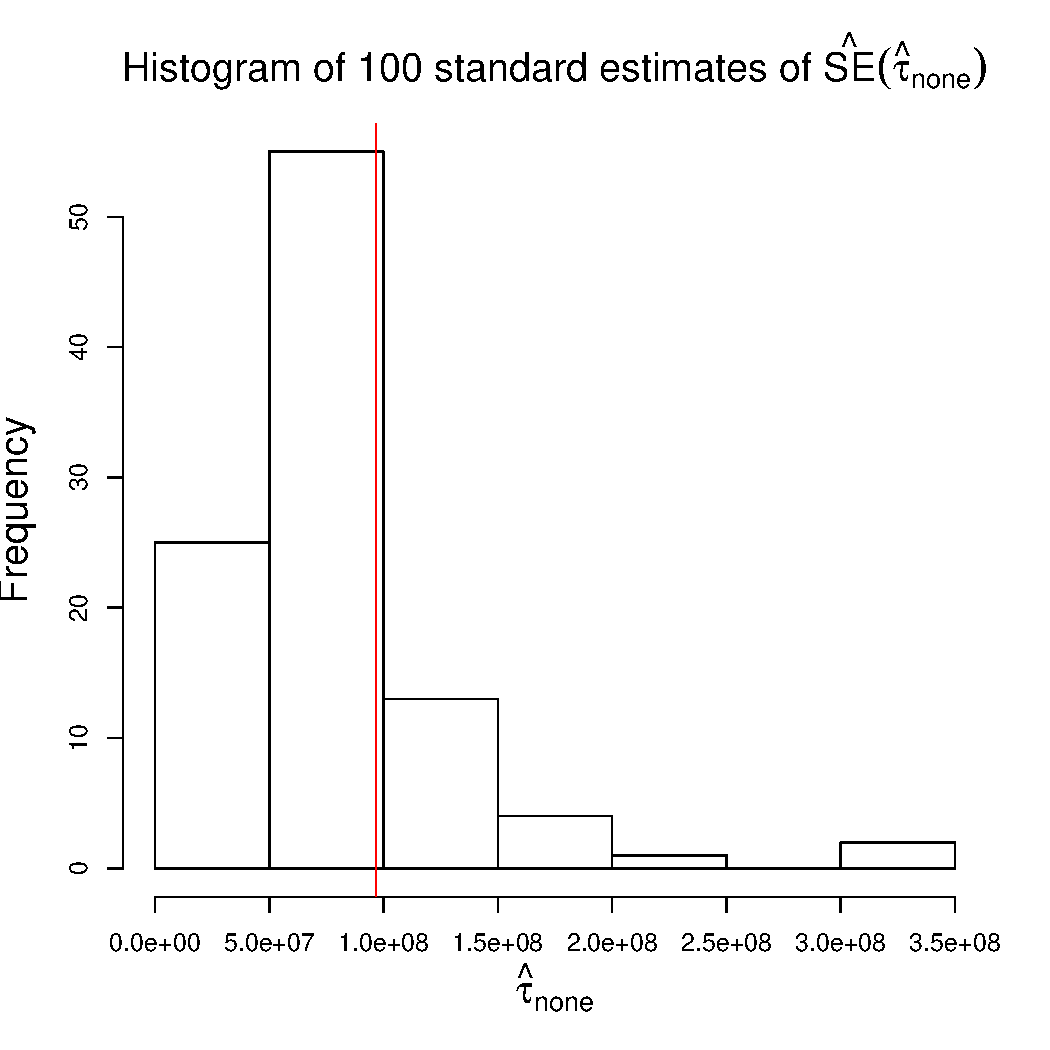
\includegraphics[width=.3\textwidth]{none_hist_se.pdf}
  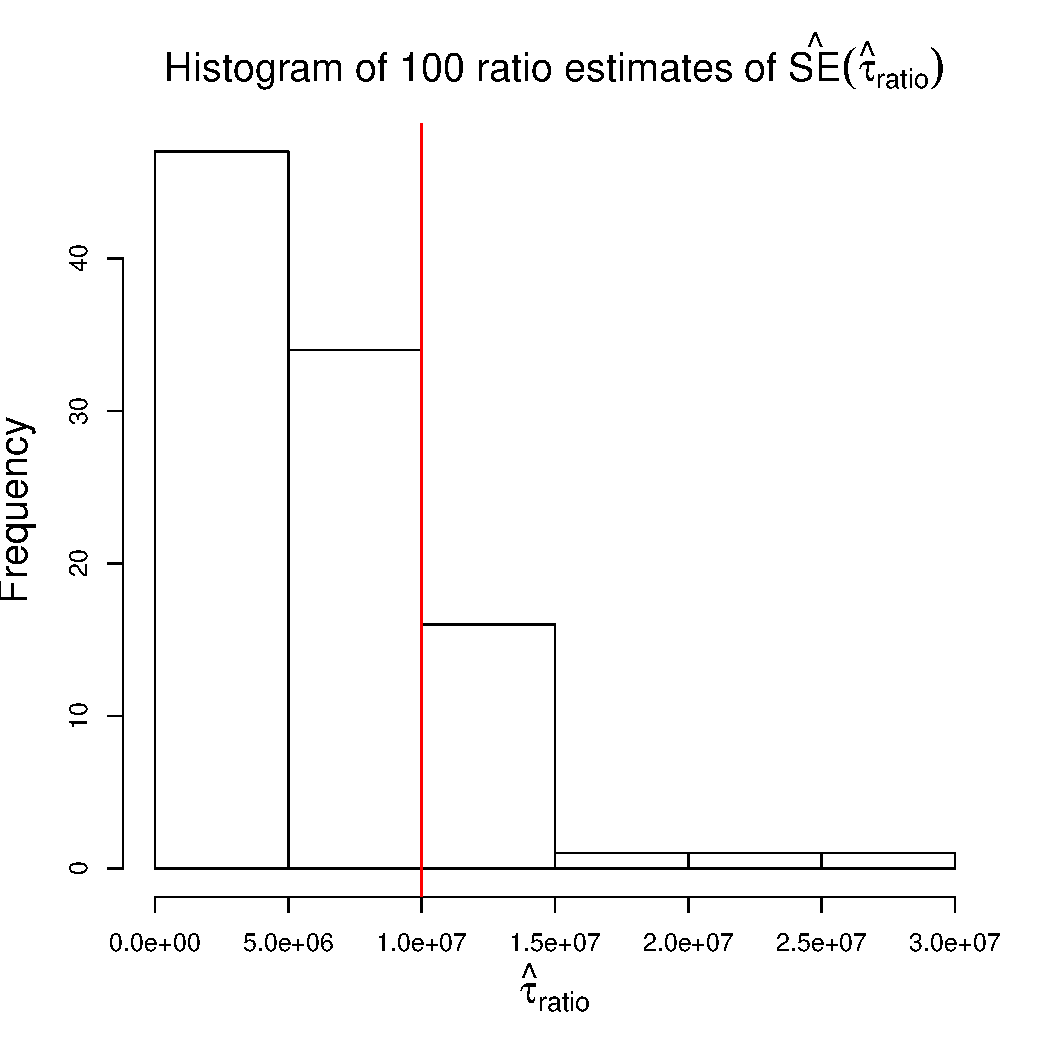
\includegraphics[width=.3\textwidth]{ratio_hist_se.pdf}
  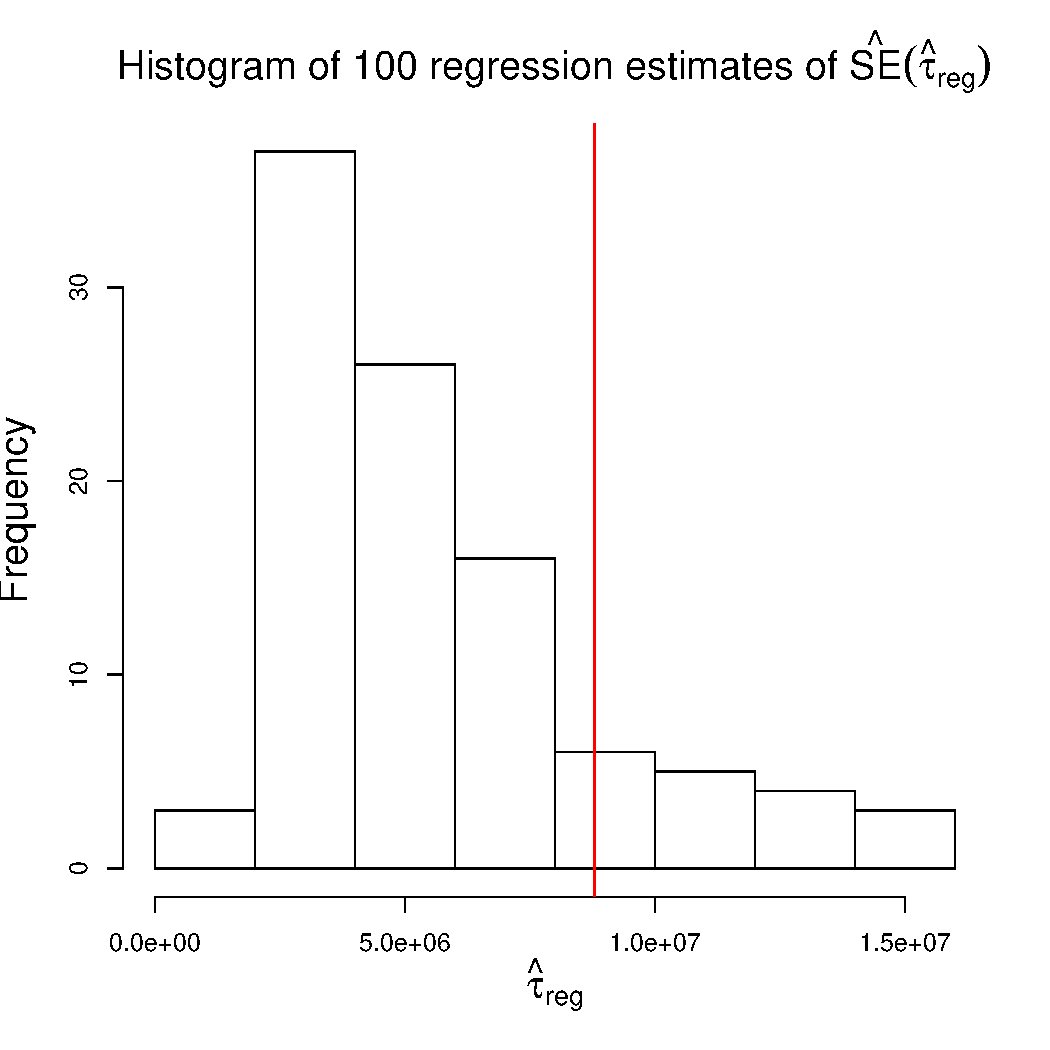
\includegraphics[width=.3\textwidth]{regression_hist_se.pdf}
    
These simulations suggest that $\hat{SE}(\hat \tau)$ is heavily right skewed in each case.  Hence, it is not suprising that we obtained an underestimate for the standard error for each of our estimators.
This could be due to the fact that the population $(y_i)$ is heavily right skewed.  Perhaps a log transformation on $y_i$ and $x_i$ might be a more appropriate analysis?
\end{solution}

\subproblem{ Imagine that you will be using this method in the next census in 2020.  Estimate the sample size needed to estimate the total population of the U.S.~to within 5,000,000 with probability \unit[95]{\%} with this method (using the finite population correction).  Use the value of $\sigma_r^2$ from the whole 2010 census to estimate $\sigma_r^2$ for the next census. }
\begin{solution}
  If we assume that the sample mean in 2020 is normally distributed with the same standard deviation as in 2010, then if $d = 5,000,000$, in each of the three cases we can solve for $n$ in the equation $ d^2 = z^2\Var(\hat{\tau}) $.  When there is no auxiliary information we have
  $$
    d^2 = z^2 \Var(\hat\tau_{none})= z^2N^2\left(1 - \frac nN\right) \frac{\sigma^2}{n} \implies n = \left(\frac{d^2}{N^2z^2\sigma^2} + \frac 1N\right)^{-1} \approx 3077.9061 
  $$

  For the ratio estimator, if we assume the approximation for the variance of $\hat\tau$ is exact, then a similar calculation gives
  $$
    d^2 = z^2 \Var(\hat\tau_{ratio})= z^2N^2\left(1 - \frac nN\right) \frac{\sigma_r^2}{n} \implies n = \left(\frac{d^2}{N^2z^2\sigma_r^2} + \frac 1N\right)^{-1} \approx 1054.4272 
  $$
  where
  $$
    \sigma_r^2 = \frac1{N-1}\sum_{i=1}^N\left(y_i - \frac{\tau_y}{\tau_x}x_i\right)^2.
  $$
  Finally, for the regression estimator, under the same approximation assumption,
  $$
    d^2 = z^2 \Var(\hat\tau_{reg})= z^2N^2\left(1 - \frac nN\right) \frac{\sigma_{reg}^2}{n} \implies n = \left(\frac{d^2}{N^2z^2\sigma_{reg}^2} + \frac 1N\right)^{-1} \approx 882.2721 
  $$
  where
  $$
    \sigma_{reg}^2 = \frac{1}{N-1}\sum_{i=1}^Nr_i^2
  $$
  and $r_i^2$ are the residuals of the least square fit from the population.

  Note that each of these is much higher than 100.  In fact, for the non-auxilary sample we might as well do the census as our normal approximation is likely not valid anymore, since the required sample size is a significant proportion of $N=3143$.

\end{solution}

\subproblem{ Do a simulation to estimate the bias and standard deviations of the ratio and regression estimators for sample size $n=100$.  Compare the bias of the ratio estimator to the estimate derived in problem 4 from Chapter 7 (above).  Compare the standard deviations to the approximate theoretical values in part (d). }

\begin{solution}
We extend the simulation carried out in (b) to $N=10^5$.  That is, we take $N$ size $n=100$ samples the population and calculate ratio and regression estimators $\hat\tau_{ratio}$ and $\hat\tau_{reg}$.  From these simulations we estimate the bias by subtracting $\tau_y$ from the mean of the samples.  We estimate the standard deviation by calculating the standard deviation of the simulated estimates. Based on problem 4, we can approximate the bias as
$$
  \mathrm{Bias}_{lin}(\hat\tau) = N\mu_x \mathrm{Bias}_{lin}(r) = N\frac{\mu_y}{\mu_x^2} \Var(\bar x)- \frac{N}{\mu_x} \Cov(\bar x, \bar y)
$$ 
where (Thompson 7.3)
$$
  \Var(\bar x) = \left(1-\frac nN\right)\frac{\sigma^2_x}{n} \quad\text{ and }\quad \Cov(\bar x,\bar y) = \left(1-\frac nN\right) \frac1n \sum_{i=1}^N \frac{(x_i-\mu_x)(y_i-\mu_y)}{N-1}.
$$

A summary of the results are given in the following histograms and summary statistic tables.
The red lines indicate the known population parameter values.

  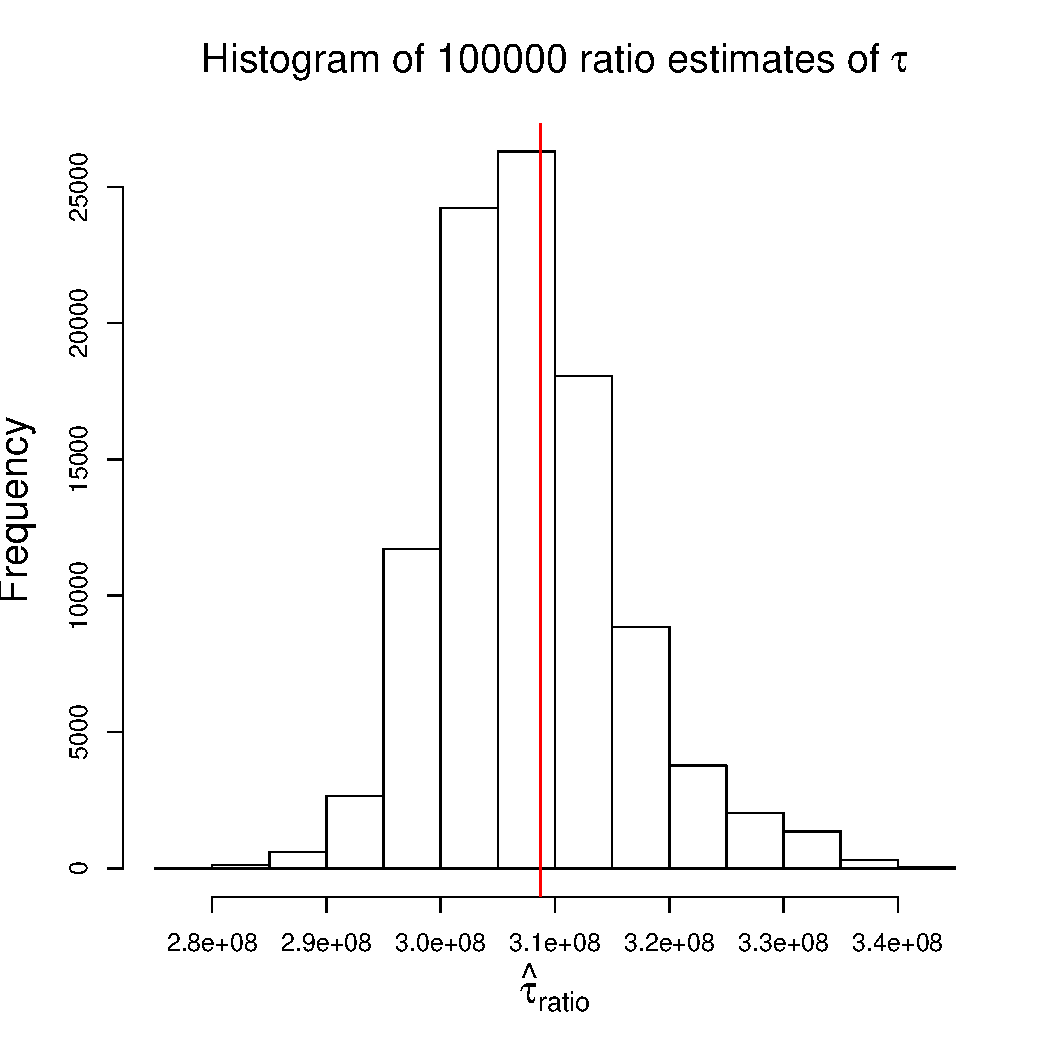
\includegraphics[width=.45\textwidth]{ratio_hist_big.pdf}
  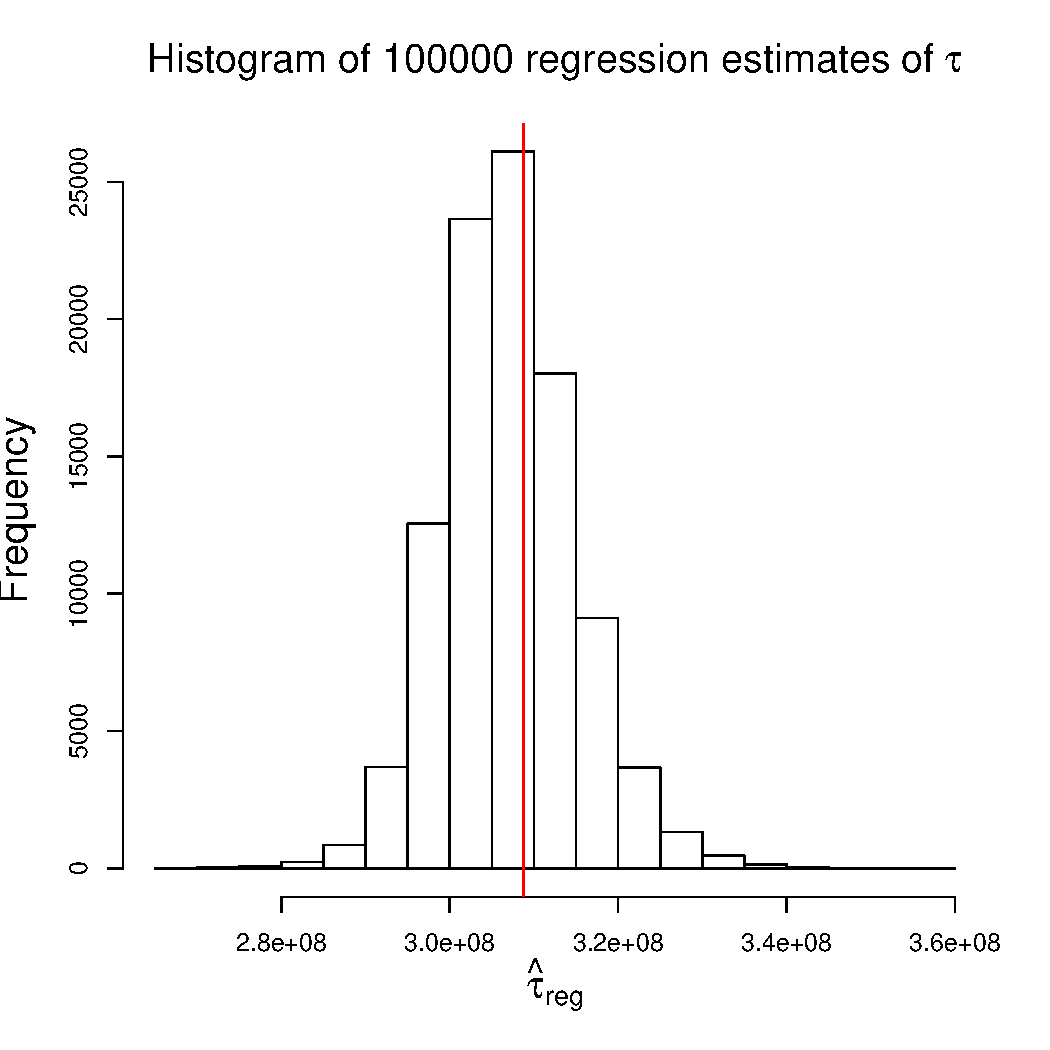
\includegraphics[width=.45\textwidth]{regression_hist_big.pdf}


\begin{center}
\renewcommand{\arraystretch}{1.3}
\begin{tabular}{c| r r}
				      &   ratio & regression \\ \hline
$\hat{\mathrm{Bias}}_{sim}(\hat\tau)$ & -980225 &   -1693615 \\
$\hat{\mathrm{Bias}}_{lin}(\hat\tau)$ &$26882270^*$&            \\
$\hat\sigma_{sim}$		      & 8145931 &    7922776 \\
\end{tabular}
\end{center}

\textsuperscript{*}The extreme value for the linearized bias is likely not
accurate.  I speculate that this is due to the extreme skew of the distribution
of the population $x_i$ that leads to a very large $\Var(\bar x) \approx
1.2\times10^8$.  In Taylor's formula, the convergence depends heavily on how
close $\bar x$ is to $\mu_x$ and $\bar y$ is to $\mu_y$.  In our highly skewed
distribution, $\mu_x^2 \ll E(\mu_x - \bar x)^2$, and it might take higher order
$n$ so that negative terms $\mu_x^{-n}E(\mu_x - \bar x)^n$ and other similar terms
involving $\mu_y$ and $E(\mu_y - \bar y)$ to observe convergence (The convergence is oscillatory in the function $y/x$ as $n$ increases).  That is,
many more terms in the Taylor series may be necessary for the approximation to
be valid.  It is also quite possible I made a mistake that I did not find.
\end{solution}

\subproblem{ This looks like a situation where PPS sampling with replacement would do well (where the size variable is the number of housing units).  Compute the theoretical standard deviation of the PPS estimator for $n=100$.  What would be the disadvantage of this sampling plan versus SRS? }
\begin{solution}
  In PPS sampling, the variance of the theoretical estimator is given by
  $$
    \sqrt{\Var(\hat \tau_p)} = \sqrt{\frac 1n\sum_{i=1}^N p_i\left(\frac{y_i}{p_i} - \tau\right)^2} \approx 2755859 = 2.76\times10^6
  $$
  where $p_i = x_i/\tau_x$.  This is much better than $\SD(\hat\tau_{ratio})
  \approx 10.0\times10^6$ and $\SD(\hat\tau_{reg})\approx 8.79\times10^6$.  One
  disadvantage of this plan is that it gives a heavy bias toward large
  counties.  This might not be appropriate if we have multiple purposes for our census, i.e.~are doing more than just estimating the total population.
  \end{solution}

\begin{longproblem}
  Unequal probability sampling is often unavoidable, so it is important to recognize when it occurs and to collect adequate information from respondents to calculate inclusion probabilities.  For example, one method of surveying anglers on a stretch of river is to place questionnaire postcards on all cars parked along the road.  An important question is then the probability of inclusion for each respondent; an analysis which ignores the differing probabilities of inclusion can bias estimates of parameters of interest (such as proportion of fly fishers, average number of fish caught, average age of anglers, etc.).  

  So suppose we are interested in anglers who fish a certain stretch of a river over a 4-week period.  The first decision is what is the sampling unit -- is it an individual angler or a trip by an individual angler?  For practical reasons in computing inclusion probabilities, it is easier if we consider each separate trip by an angler as a separate unit.  Therefore, an angler who fishes on 4 separate days during this time period contributes 4 angler-trips to the population.  Second, we have to decide how to deal with multiple people coming in one vehicle; we'll assume that every individual in a vehicle is asked to fill out a questionnaire.  We should also recognize that we're ignoring people who fish this stretch of river, but don't park their vehicle there (floaters, for example).  Perhaps we could restrict our population to bank anglers.  These and related issues are all important to address before we design the survey.

  Now, suppose I am designing a survey of this stretch of the river.  I have decided that I will restrict my population to those anglers who arrive in a vehicle that is parked along this stretch sometime between 0600 hours and 2100 hours (6am to 9pm) each day during these 4 weeks.  My plan is as follows: I will randomly select 3 of the 8 weekend days during this period and 5 of the 20 weekdays.  On each selected day, I will randomly (and independently of other days) select one of the two starting times: 6am or 11am.  

  After I select one of the two start times, I will select a random starting place for my route in the following way: It takes me 7 hours to drive the stretch from south to north at a steady pace, distributing postcards and 3 hours to drive from the north end to the south if I'm not distributing postcards.  So imagine a loop starting at the south end at 0 hours, reaching the north end at 7 hours and returning to the south end at 10 hours.  Since I go at a steady pace (assume the time to distribute postcards is negligible), after 3.5 hours, for example, I will be halfway between south and north; after 6 hours I will be 6/7 of the way from the south to north, and after 8.5 hours I will be halfway along the route, heading south.  Now I pick a random time from 0 to 10 hours and I start at the point on the route that that would put me.  For example, if I picked 2.2 hours, then I would start 2.2/7 of the way from the south end. I would then continue north for 4.8 hours until I reached the north end, return to the south end (without distributing postcards) at 7.8 hours, then complete the rest of the route to my starting place.  If I randomly picked 8.5 hours, then I would imagine starting 1.5 hours after my start time to actually start the route at the south end.  In this way the entire route is driven exactly once.
  
  Assume the time to distribute postcards is negligible; Thus, I will work either the period 0600-1600 or 1100-2100.
  
  In order to calculate the inclusion probability for a selected angler, I will need to know the time his or her vehicle arrived and the time it left on the day the angler received a survey, so that will be one of the questions I ask on the questionnaire.  Recall also that inclusion probabilities are computed from this perspective: before I select the days, starting points and starting times, what is the probability that an angler who is parked along the river tween times $t_1$ and $t_2$ on a specific day will be included in the survey?
  
  Compute the inclusion probabilities for the following anglers:
  \begin{enumerate}[(a)]
    \item Jeff: parked from 0500 to 1030 on Thursday of week 2.
    \item Ellen: parked from 0930 to 1700 on Sunday of week 3.
    \item Iris: parked from 1700 to 2200 on Monday of week 4.
  \end{enumerate} 

  It may help to draw a graph with time on the x-axis and location long the river on the y-axis.  Then a parked car is a horizontal line segment and the worker (me) is a diagonal line segment with a random start time and a random start point.  The probability of inclusion is the probability that the worker's segment intersects the angler's segment times the probability this is one of the chosen days.  Actually, the worker will be represented by two separate line segments (why?). ANS: One segment is from where you start to the end, the other is from the beginning of the river to the end of the day.
\end{longproblem}

\begin{solution}
  If we assume that the selection of the days to survey and the time/location along the
  river are independent, then the probability that any angler trip is surveyed
  is given by the probability that they are intercepted on a trip multiplied by
  the probability that that the day of their trip is selected.  The probability
  of selecting any one weekday is the number of samples of size 5 that include
  the given weekday divided by the total number of samples.  That is,  
  $\left.\binom{19}4 \middle / \binom{20}5\right. = \frac 14$.  
  Similarly, the probability of choosing any one weekend day is 
  $\left. \binom 72 \middle/\binom 83\right. =\frac 38$. 

  Suppose a day and a shift has been selected. We wish to calculate the
  probability that we survey a given angler with a given time spent fishing
  \emph{during the driving shift}, say $h$.
  For now, assume that their car is parked at the end of the river and they
  begin fishing at the beginning of the shift.  Recall that we sample uniformly
  from $[0,10]$ hours which determines a location on the route to start
  driving.  Any sampled time just after $7$ will result in us missing the car
  (unless they fish for 10 hours and we catch them on the way back in which
  case the probability of surveying is 1), and for each sampled time before $7$
  until $7-h$ (mod 10 if $h>7$) we will survey their car. Hence, the width of the
  interval of time/locations is $h$ and the probability of selection is $h/10$.

  Now, note that if the angler does not start fishing at the beginning of the
  shift, then the latest time/location in which we catch them ($7$ in the last
  case), say $b$, and the earliest time, say $a$, ($7-h$ in the last case) are
  merely shifted back by the amount of time determined by the steady rate at
  which we drive.  Regardless of this shift, the assumption of  consistent
  driving rate along the river preserves the width of the interval $[a,b]$,so the 
  probability that  we survey the car is still $h$.  Moreover, if the location of the angler is
  further down river, a similar shift of the interval occurs and preserves the
  interval width.  In all cases, the probability of survey given a shift
  and this day being selected in the survey, is $h/10$.

  Finally, to take into account the driving shift, we note that selecting
  a morning shift or an evening shift are disjoint events.  Hence, if we denote
  $E_{a}$ as the event of surveying a given angler $a$, and $M$ the event
  that we select a morning shift, then the law of total probability says
  $$
    P(E_a) = P(E_a|M)P(M) + P(E_a|M^c)P(M^c).
  $$
  We can now calculate the inclusion probabilities of the three given anglers. For Jeff, $h = 10.5 - 6 = 4.5$, so
  $$
    P(\text{Jeff surveyed}) = \frac 1{4} \left( \frac{4.5}{10}\cdot \frac 12 + 0 \frac12\right) = \frac{9}{160} = 0.056
  $$
  For Ellen, she has $h_1 = 16 - 9.5 = 6.5$ hours in the morning shift and $h_2 = 17-11 = 6$ hours in the evening, so
  $$
    P(\text{Ellen surveyed}) = \frac 3{8} \left( \frac{6.5}{10}\cdot \frac 12 + \frac6{10}\cdot \frac12\right) = \frac{15}{64} = 0.234 
  $$
  For Iris, she has $h = 21 - 17 = 4$ hours in the evening shift, so 
  $$
    P(\text{Iris surveyed}) = \frac 1{4} \left(0 \frac12  + \frac{4}{10}\cdot \frac 12\right) = \frac{1}2 = 0.05.
  $$

\end{solution}
\newpage
\problem{ Extra Credit: In Section 6.4 of Thompson, he gives a small sample $(N=3, n=2)$ of sampling with replacement with unequal probabilities where the Hansen-Hurwitz estimator $(\hat \tau_p)$ of the population total had much smaller variance than the Horvitz-Thompson estimator $(\hat\tau_\pi)$.  Create an example of this same size, where the reverse is true. }
\begin{solution}
  In circumstances similar to the ``circus statistician'', if we have a population as follows


\begin{center}
\renewcommand{\arraystretch}{1.3}
\begin{tabular}{c| r r r}
\hline
$y_i$ & .01 & .01 & 50000\\
$p_i$ & .00005 & .00005 & .9999\\
\hline
\end{tabular}
\end{center}

Then, a summary table similar to Thompson's is as follows
\begin{center}
\renewcommand{\arraystretch}{1.3}
\begin{tabular}{l r c r r}
\hline
  $s$ &    $p(s)$  &      $y_s$      &$\hat\tau_p$&$\hat\tau_{\pi}$\\\hline
 1, 1 & 2.5000e-09 & (1e-02 , 1e-02) &   200.0 &    200.005\\
 1, 2 & 2.5000e-09 & (1e-02 , 1e-02) &   200.0 &    200.005\\
 1, 3 & 4.9995e-05 & (5e+04 , 1e-02) & 25102.5 &  50100.003\\
 2, 1 & 2.5000e-09 & (1e-02 , 1e-02) &   200.0 &    200.005\\
 2, 2 & 2.5000e-09 & (1e-02 , 1e-02) &   200.0 &    200.005\\
 2, 3 & 4.9995e-05 & (5e+04 , 1e-02) & 25102.5 &  50100.003\\
 3, 1 & 4.9995e-05 & (1e-02 , 5e+04) & 25102.5 &  50100.003\\
 3, 2 & 4.9995e-05 & (1e-02 , 5e+04) & 25102.5 &  50100.003\\
 3, 3 & 9.9980e-01 & (5e+04 , 5e+04) & 50005.0 & 100000.001\\
 Mean:&            &                 & 50000.02& 50000.02\\
 Std. Dev.:&       &                 & 352.16  & 5.182    \\
 
\hline
\end{tabular}
\end{center}

See \texttt{problem8.r} for details on how this was discovered.  Essentially, I tried to minimize $\Var(\hat\tau_\pi) - \Var(\hat\tau_p)$ to get a rough idea of where the parameters resulted in a very negative quantity.

\end{solution}

\end{document} 
